\documentclass[parskip=half]{scrartcl}

% --------------------------------------------
%       Config
% --------------------------------------------
\title{Research \\ EDA/CPE for Smart Cities}
\author{Dominik Stiller}

\usepackage[USenglish]{babel}
\usepackage[T1]{fontenc}
\usepackage[utf8]{inputenc}
\usepackage{lmodern}
\usepackage{amsmath}
\usepackage{amssymb}
\usepackage{textcomp}
\usepackage{csquotes}
\usepackage[binary-units=true]{siunitx}
\usepackage[
	backend=biber,
	bibwarn=true,
	bibencoding=utf8,
	sortlocale=en_US,
	style=ieee
]{biblatex}
\addbibresource{./litreview.bib}
\usepackage{graphicx}
\graphicspath{ {./images/} }

\begin{document}

\maketitle


% --------------------------------------------
%       Content
% --------------------------------------------

This document contains a non-exhaustive list of research for smart cities and how they use event-driven architectures and complex event processing.

\section{Applications and Stories}

Common themes:
\begin{itemize}
	\item Traffic management
	\item Parking
	\item Intelligent buildings (security, lighting, energy efficiency)
	\item Waste management
	\item Environmental monitoring
\end{itemize}

\cite[p.~2]{Morales.2015}:
\begin{itemize}
	\item Energy consumption profiles
	\item Concentration and distribution of pollutants
	\item Urban heat distribution caused by urban structures
	\item Energy efficient urban design
	\item Use of public transportation services
	\item Traffic flow of vehicles
	\item Movement of goods and freight
	\item Pedestrian's flow
	\item Use and load of telecommunication networks
	\item Presence of citizens in places of interest
	\item Livability
	\item Citizens living habits
	\item Citizen health monitoring
\end{itemize}

\cite[p.~8~ff.]{Ahmed.2018}:
\begin{itemize}
	\item Structural health: monitor cracks in buildings
	\item Smart parking: monitor free/taken parking spots
	\item Waste management: monitor trash can status
	\item Smart roads: guide citizens in traffic and detect traffic patterns
	\item Smart surveillance and intrusion detection for homes where the local police department is automatically notified
	\item Pollution monitoring
	\item Smart lighting
	\item Smart energy grid
	\item Smart industry
\end{itemize}

\cite[p.~7~f.]{Petrolo.2017}
\begin{itemize}
	\item Transport: dynamic route calculation informed of accidents and congestion
	\item Energy: reporting of faults
	\item Emergency services: detection of accidents and crimes
	\item Waste management: detection of full bins
	\item Air and water: reporting of air and water pollution
	\item Recreation: produce data on large events like concerts to inform public transport
\end{itemize}

\cite[p.~8~ff.]{Alavi.2018}:
\begin{itemize}
	\item Price calculation for EV parking lots based on energy market
	\item Status monitoring of hospital patients
	\item Monitoring and intelligent routing of ambulances
	\item Congestion control, smart parking and traffic management
	\item Smart streetlights for intelligent and weather-adaptive lighting
	\item Noise pollution monitoring
\end{itemize}

\cite[p.~209~ff.]{Angelakis.2017}:
\begin{itemize}
	\item Traffic flow management: reduce emissions, noise and travel times by monitoring and actively controlling traffic
	\item Smart grid: distributed generation and distribution (voltage stability, loss reduction), real-time energy pricing (demand response, electricity markets)
	\item Intelligent buildings: increase security and energy efficiency, automate HVAC
	\item Healthcare in residential environments:  monitor environment (temperature, humidity, luminosity...) and movements to analyze health and well-being
\end{itemize}

\cite[p.~16]{Fernandes.2012}:
\begin{itemize}
	\item Parking availability
	\item Environmental monitoring: visualize temperature, luminosity, noise, CO2 emissions on map
	\item Participatory sensing: user app collects data, users can enter events (e.g., defects, accidents) manually
	\item Precision irrigation: irrigate plants based on soil humidity, wind, and weather forecast
	\item Smart energy metering
\end{itemize}

\cite[p.~30]{Presser.2014}:
\begin{itemize}
	\item Public parking space availability prediction
	\item Real-time 3D maps of power consumption, public transport,... (real-live version of SimCity)
	\item Neighbor vote for turning on/off nearby street lamps
	\item Redirect cars or suggest public transport in case of high air pollution
	\item 101 other scenarios which have been considered are listed in \cite{CityPulseConsortium.2020}
\end{itemize}

\cite[p.~1]{Garcia.2020}:
\begin{itemize}
	\item Precision irrigation for agriculture and city parks based on soil measurements and weather
\end{itemize}

\cite{Wahner.2019}:
\begin{itemize}
	\item Anomaly detection in real-time for 100,000+ connected cars, full solution is available on GitHub
\end{itemize}


\section{Event Definitions}

\enquote{Geo-event: An occurrence of a change of state associated to a phenomenon of interest ($\mathbb{D}_p$), and which is related to a geographic location ($\mathbb{D}_s$) and a specific time ($\mathbb{D}_t$).}~\cite[p.~3]{Morales.2015}

\begin{align*}
	\mathbb{D}_p &= \{name: value, phenomena: [value_1, value_2, ..., value_n], condition: value\} \\
	\mathbb{D}_s &= \{extent: value, granularity: value\} \\
	\mathbb{D}_t &= \{time-window: value, granularity: value\}
\end{align*}


\section{Available Data}

\cite{CityPulse.2015} (historic):
\begin{itemize}
	\item Road Traffic
	\item Pollution
	\item Weather
	\item Cultural/Social/Library Events
	\item Parking
\end{itemize}

\cite{HelsinkiRegionalTransportAuthority.2020} (real-time):
\begin{itemize}
	\item Public transport vehicle position
	\item Arrivals and departures
	\item Driver changes
\end{itemize}

\cite{data.gov.sg.2020} (real-time):
\begin{itemize}
	\item Air quality
	\item Carpark availability
	\item Taxi availability
	\item Weather measurements (temperature, humidity, precipitation, wind, UV radiation)
	\item Weather forecast
	\item Traffic images
\end{itemize}


\section{Challenges}
\enquote{Geoprocessing of data streams inherits challenges from big data analysis: volume, velocity, variety, value, and veracity.}~\cite[p.~1]{Morales.2015}

\cite[p.~2~ff.]{Ahmed.2018}:
\begin{itemize}
	\item High cost and long development tmie \textrightarrow private--public collaboration and common platform
	\item Choice of communication paradigm (continuous, random, incremental) \textrightarrow hierarchical structure
	\item Sustainability of network and compatibility of devices
	\item No best practices for IT platforms
\end{itemize}

\cite[p.~9~f.]{Petrolo.2017}:
\begin{itemize}
	\item Big data: efficient query and storage and extraction of meaning
	\item Privacy
	\item Security: threats from cyber-terrorism/-vandalism
\end{itemize}


\section{Architectures}

\begin{figure}
	\centering
	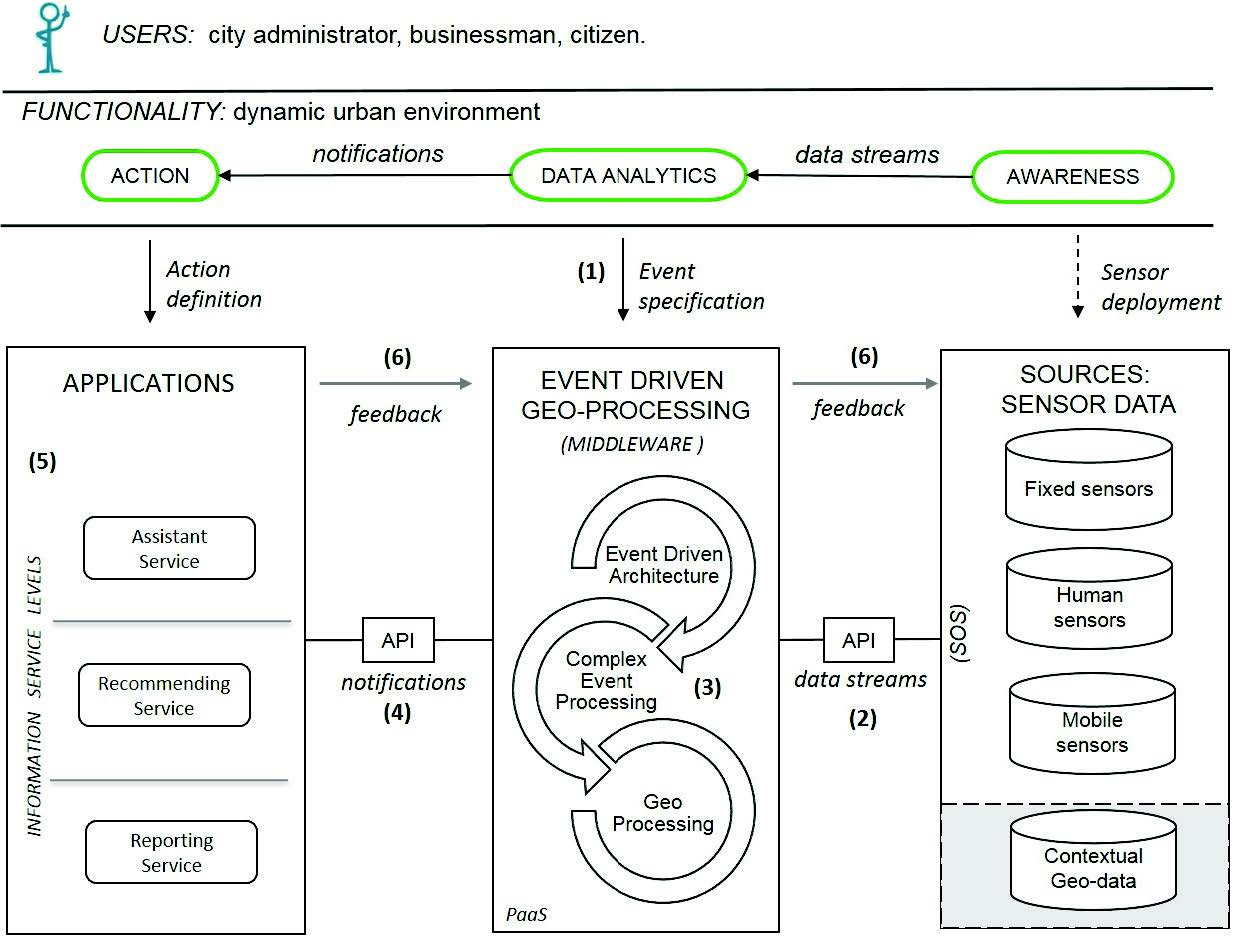
\includegraphics[width=\textwidth]{Morales_2015}
	\caption{Event-driven geoprocessing system architecture~\cite[p.~3]{Morales.2015}}
	\label{fig:morales-arch}
\end{figure}

\begin{figure}
	\centering
	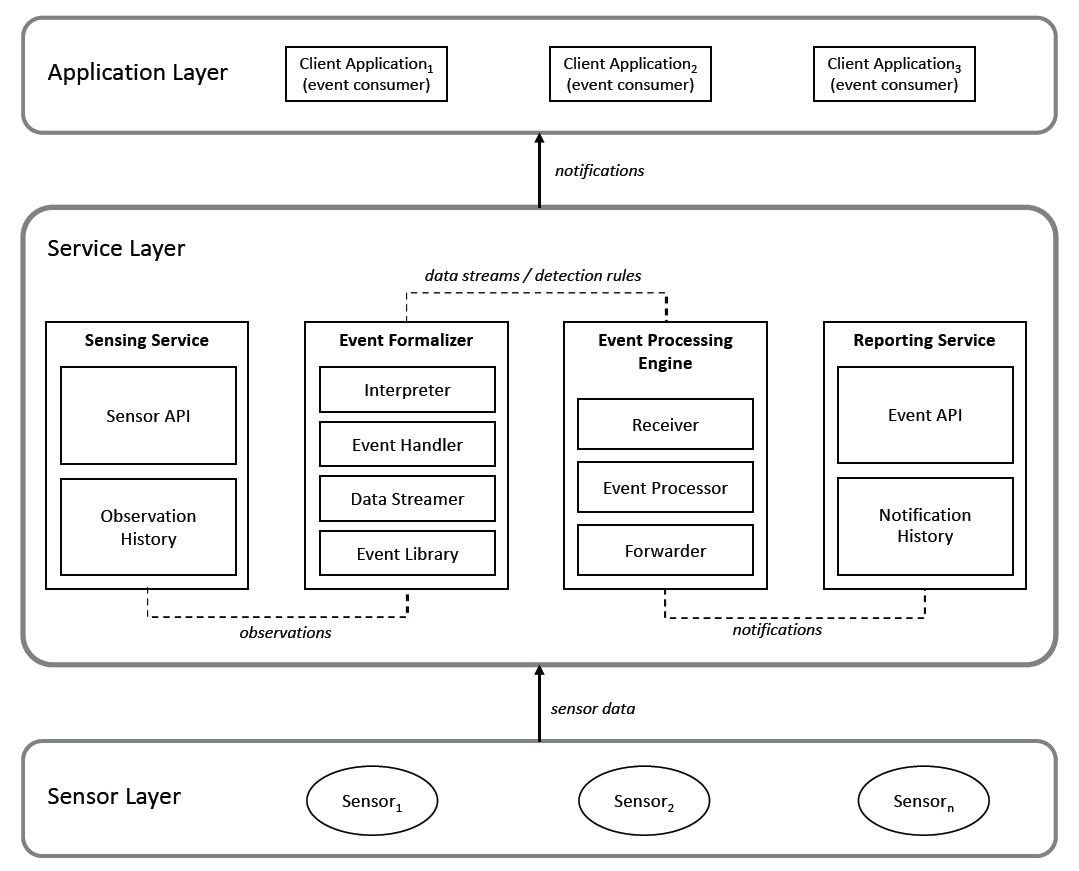
\includegraphics[width=\textwidth]{Garcia_2019a}
	\caption{Reference Architecture for Smart City Applications (RASCA)~\cite[p.~12]{GarciaAlvarez.2019}}
	\label{fig:rasca}
\end{figure}

\begin{figure}
	\centering
	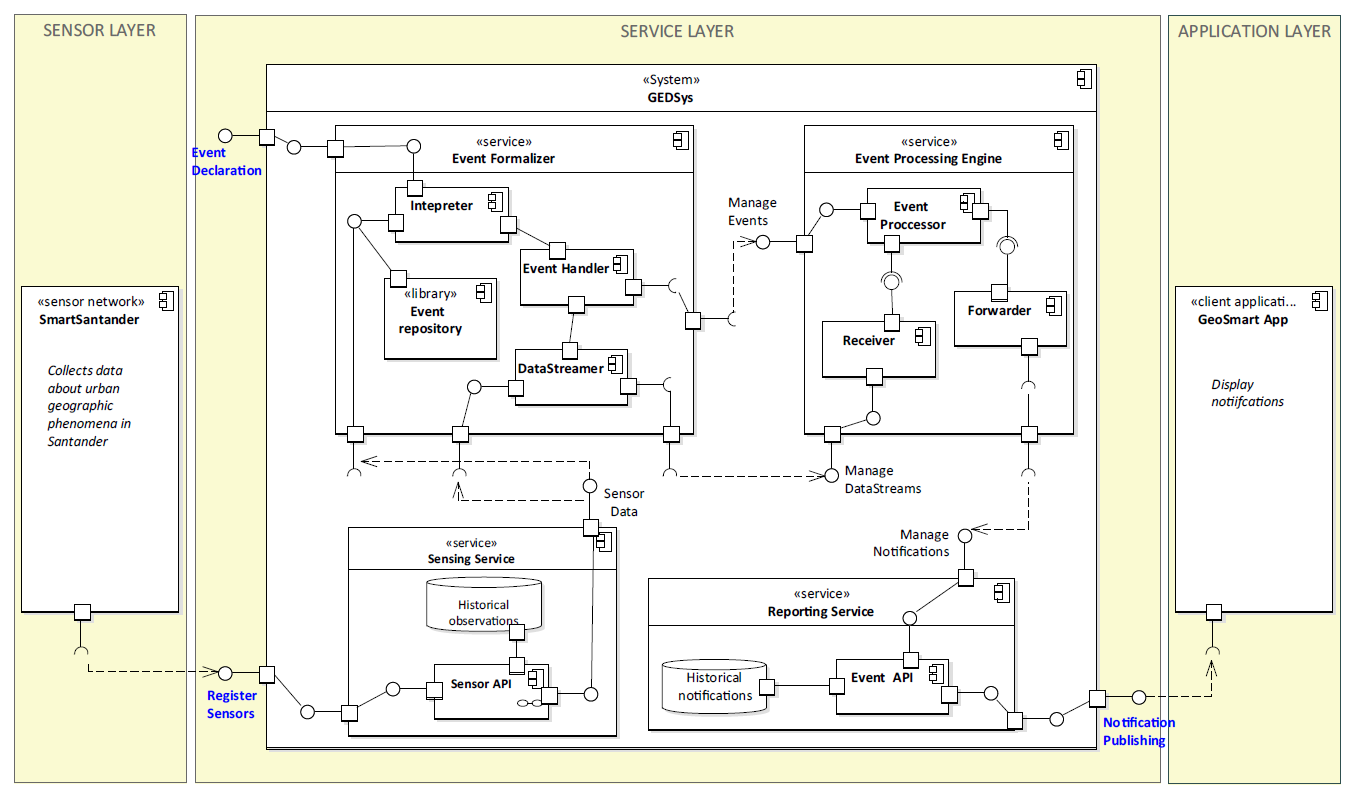
\includegraphics[width=\textwidth]{Garcia_2019b}
	\caption{Implementation of RASCA~\cite[p.~13]{GarciaAlvarez.2019}}
	\label{fig:rasca-impl}
\end{figure}

The architecture in figures \ref{fig:rasca} and \ref{fig:rasca-impl} is an instantiation of the reference architecture in figure \ref{fig:morales-arch} and was used with data from SmartSantander project to detect geospatial events, e.g. temperature above \SI{0}{\celsius} in the city center. \cite{GarciaAlvarez.2019} mentions that Flink has good throughput but no geospatial matching capabilities. 

\begin{figure}
	\centering
	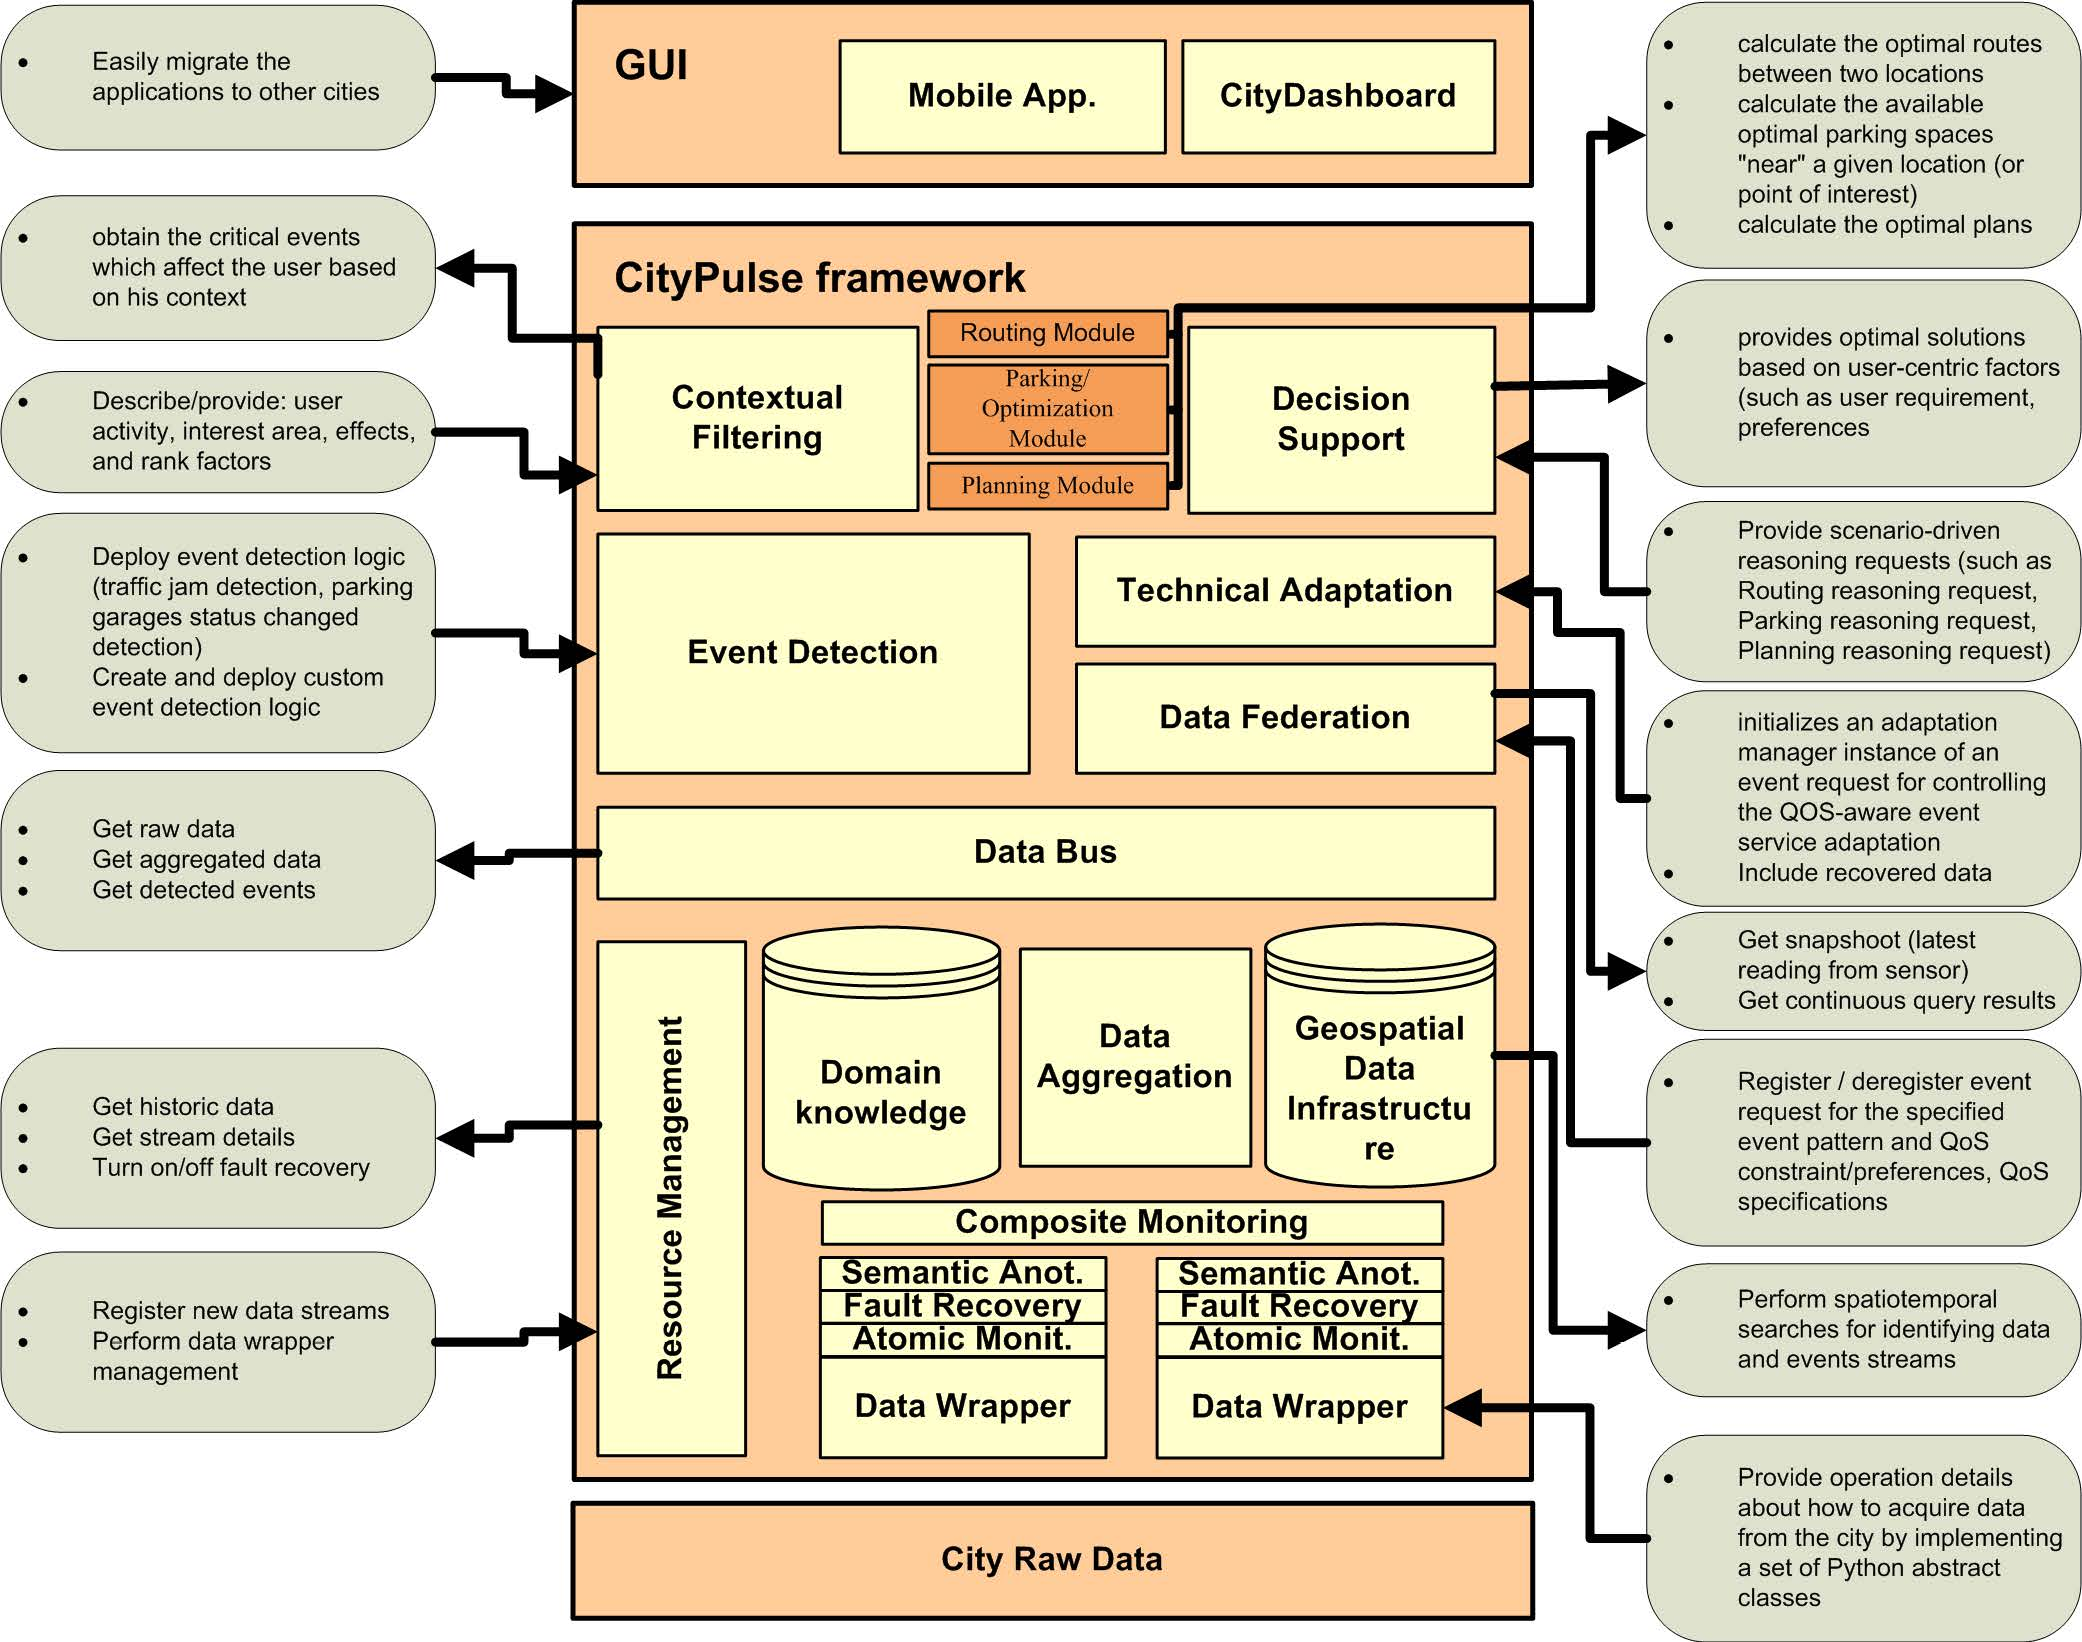
\includegraphics[width=\textwidth]{Tsiatsis_2015b}
	\caption{Smart City Framework for CityPulse~\cite[p.~39]{Tsiatsis.2015}}
	\label{fig:citypulse-framework}
\end{figure}

\begin{figure}
	\centering
	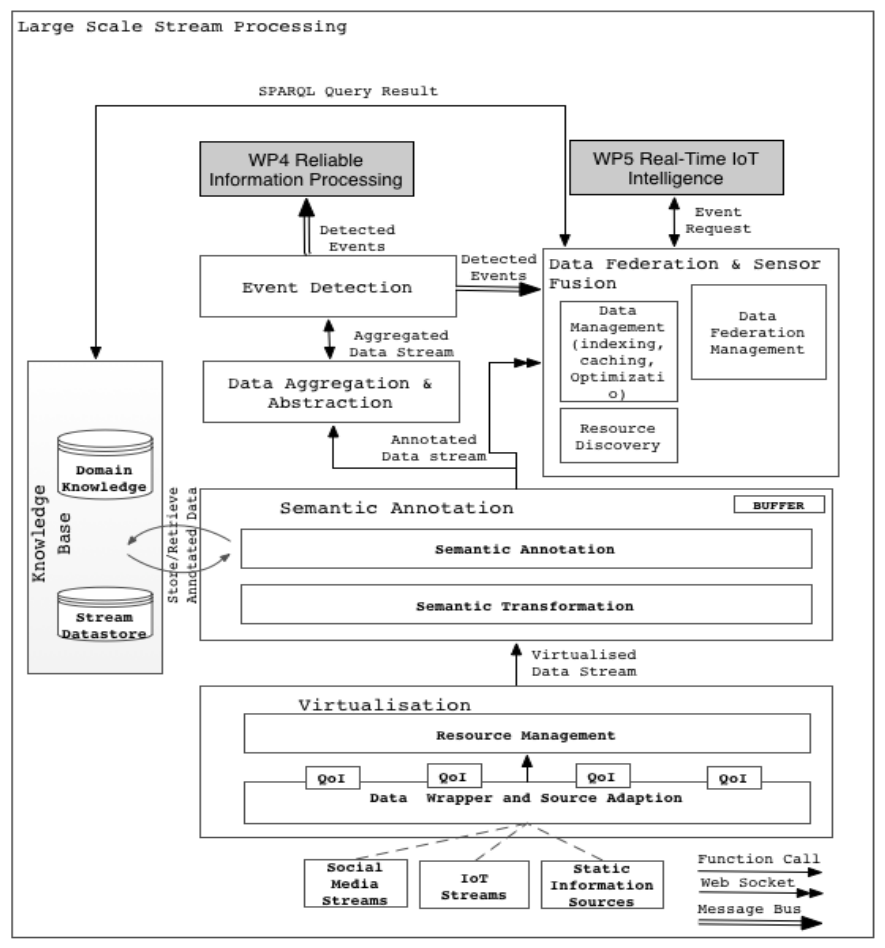
\includegraphics[width=\textwidth]{Tsiatsis_2015}
	\caption{Large Scale Data Analysis Functional Group for CityPulse~\cite[p.~25]{Tsiatsis.2015}}
	\label{fig:citypulse-streaming}
\end{figure}

The CityPulse project described in \cite{Tsiatsis.2015, Presser.2014, Presser.2016, Puiu.2016, Puiu.2016b} uses AMQP for message transport. The overall architecture is shown in figure \ref{fig:citypulse-framework} while the stream processing is shown in figure \ref{fig:citypulse-streaming}.


\clearpage
\printbibliography

\end{document}
